\section{DGN-NO-ACT:  Towards Interpretability and Performance}\label{sec:dgn-no-act}

\begin{figure}
\centering
\begin{minipage}{0.8\columnwidth}
\centering
\begin{minipage}{0.49\columnwidth}
\resizebox{1.0\columnwidth}{!}{
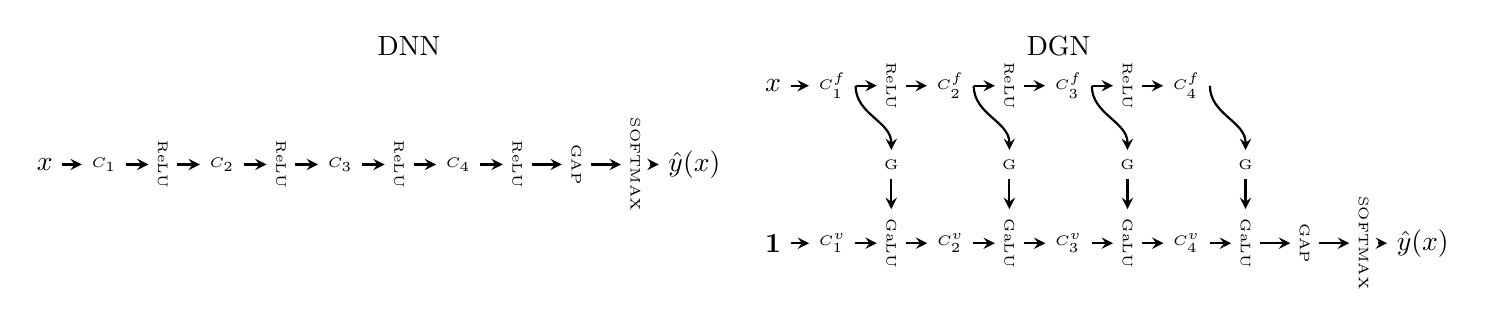
\begin{tikzpicture}
\node []  (dnn-text)at (-4.125,2) {DNN};

\node []  (dnn-output) at (-0.5,0.5) {$\hat{y}(x)$};
\node [rotate=-90]  (dnn-smax) at (-1.25,0.5) {\tiny{SOFTMAX}};
\draw [-stealth,thick]   (dnn-smax.north) -- (dnn-output.west);

\node [rotate=-90]  (dnn-gap) at (-2,0.5) {\tiny{GAP}};
\draw [-stealth,thick]   (dnn-gap.north) -- (dnn-smax.south);

\node [rotate=-90] (dnn-relu-4) at (-2.75,0.5){\tiny{ReLU}};
\node [] (dnn-c4) at (-3.5,0.5){\tiny{$C_4$}};
\draw [-stealth,thick]   (dnn-c4.east) -- (dnn-relu-4.south);
\draw [-stealth,thick]   (dnn-relu-4.north) -- (dnn-gap.south);



\node [rotate=-90] (dnn-relu-3) at (-4.25,0.5){\tiny{ReLU}};
\node [] (dnn-c3) at (-5,0.5){\tiny{$C_3$}};
\draw [-stealth,thick]   (dnn-c3.east) -- (dnn-relu-3.south);
\draw [-stealth,thick]   (dnn-relu-3.north) -- (dnn-c4.west);


\node [rotate=-90] (dnn-relu-2) at (-5.75,0.5){\tiny{ReLU}};
\node [] (dnn-c2) at (-6.5,0.5){\tiny{$C_2$}};
\draw [-stealth,thick]   (dnn-c2.east) -- (dnn-relu-2.south);
\draw [-stealth,thick]   (dnn-relu-2.north) -- (dnn-c3.west);

\node [rotate=-90] (dnn-relu-1) at (-7.25,0.5){\tiny{ReLU}};
\node [] (dnn-c1) at (-8,0.5){\tiny{$C_1$}};
\draw [-stealth,thick]   (dnn-c1.east) -- (dnn-relu-1.south);
\draw [-stealth,thick]   (dnn-relu-1.north) -- (dnn-c2.west);



\node [] (dnn-input) at (-8.75,0.5){$x$};
\draw [-stealth,thick]   (dnn-input.east) -- (dnn-c1.west);


%%%%%%%%%%%%%%%%%%%%%%%%%%%%%%%%%%%%%%%%%%%%%%%%%%%%%%%%%%%%%%%%%
\node []  (fntext)at (4.125,2) {DGN};

%\node []  (output) at (7.5,1.5) {$\hat{y}(x)$};


\node [] (dgn-f-c4) at (5.75,1.5){\tiny{$C^{\text{f}}_4$}};


\node [rotate=-90] (dgn-relu-3) at (5,1.5){\tiny{ReLU}};
\node [] (dgn-f-c3) at (4.25,1.5){\tiny{$C^{\text{f}}_3$}};
\draw [-stealth,thick]   (dgn-f-c3.east) -- (dgn-relu-3.south);
\draw [-stealth,thick]   (dgn-relu-3.north) -- (dgn-f-c4.west);


\node [rotate=-90] (dgn-relu-2) at (3.5,1.5){\tiny{ReLU}};
\node [] (dgn-f-c2) at (2.75,1.5){\tiny{$C^{\text{f}}_2$}};
\draw [-stealth,thick]   (dgn-f-c2.east) -- (dgn-relu-2.south);
\draw [-stealth,thick]   (dgn-relu-2.north) -- (dgn-f-c3.west);


\node [rotate=-90] (dgn-relu-1) at (2,1.5){\tiny{ReLU}};
\node [] (dgn-f-c1) at (1.25,1.5){\tiny{$C^{\text{f}}_1$}};
\draw [-stealth,thick]   (dgn-f-c1.east) -- (dgn-relu-1.south);
\draw [-stealth,thick]   (dgn-relu-1.north) -- (dgn-f-c2.west);



\node [] (dgn-f-input) at (0.5,1.5){$x$};
\draw [-stealth,thick]   (dgn-f-input.east) -- (dgn-f-c1.west);

\node []  (dgn-output) at (8.75,-0.5) {$\hat{y}(x)$};
\node [rotate=-90] (dgn-smax) at (8,-0.5){\tiny{SOFTMAX}};
\draw [-stealth,thick]   (dgn-smax.north)--(dgn-output.west);

\node [rotate=-90] (dgn-gap) at (7.25,-0.5){\tiny{GAP}};
\draw [-stealth,thick]   (dgn-gap.north)--(dgn-smax.south);



\node [rotate=-90] (dgn-galu-4) at (6.5,-0.5){\tiny{GaLU}};
\draw [-stealth,thick]   (dgn-galu-4.north) -- (dgn-gap.south);

\node [] (dgn-v-c4) at (5.75,-0.5){\tiny{$C^{\text{v}}_4$}};
\draw [-stealth,thick]   (dgn-v-c4.east) -- (dgn-galu-4.south);

\node [rotate=-90] (dgn-galu-3) at (5,-0.5){\tiny{GaLU}};
\node [] (dgn-v-c3) at (4.25,-0.5){\tiny{$C^{\text{v}}_3$}};
\draw [-stealth,thick]   (dgn-v-c3.east) -- (dgn-galu-3.south);
\draw [-stealth,thick]   (dgn-galu-3.north) -- (dgn-v-c4.west);



\node [rotate=-90] (dgn-galu-2) at (3.5,-0.5){\tiny{GaLU}};
\node [] (dgn-v-c2) at (2.75,-0.5){\tiny{$C^{\text{v}}_2$}};
\draw [-stealth,thick]   (dgn-v-c2.east) -- (dgn-galu-2.south);
\draw [-stealth,thick]   (dgn-galu-2.north) -- (dgn-v-c3.west);


\node [rotate=-90] (dgn-galu-1) at (2,-0.5){\tiny{GaLU}};
\node [] (dgn-v-c1) at (1.25,-0.5){\tiny{$C^{\text{v}}_1$}};

\draw [-stealth,thick]   (dgn-v-c1.east) -- (dgn-galu-1.south);
\draw [-stealth,thick]   (dgn-galu-1.north) -- (dgn-v-c2.west);




\node [] (dgn-input) at (0.5,-0.5){$\mathbf{1}$};
\draw [-stealth,thick]   (dgn-input.east) -- (dgn-v-c1.west);




\node[] (dgn-gating-1) at (2,0.5){\tiny{G}};
\draw [-stealth,thick]   (dgn-f-c1.east) to[out=-90,in=90] (dgn-gating-1.north);
\draw [-stealth,thick]   (dgn-gating-1.south) -- (dgn-galu-1.west);


\node[] (dgn-gating-2) at (3.5,0.5){\tiny{G}};
\draw [-stealth,thick]   (dgn-f-c2.east) to[out=-90,in=90] (dgn-gating-2.north);
\draw [-stealth,thick]   (dgn-gating-2.south) -- (dgn-galu-2.west);



\node[] (dgn-gating-3) at (5,0.5){\tiny{G}};
\draw [-stealth,thick]   (dgn-f-c3.east) to[out=-90,in=90] (dgn-gating-3.north);
\draw [-stealth,thick]   (dgn-gating-3.south) -- (dgn-galu-3.west);


\node[] (dgn-gating-4) at (6.5,0.5){\tiny{G}};
\draw [-stealth,thick]   (dgn-f-c4.east) to[out=-90,in=90] (dgn-gating-4.north);
\draw [-stealth,thick]   (dgn-gating-4.south) -- (dgn-galu-4.west);

	
\end{tikzpicture}


}
\end{minipage}
\begin{minipage}{0.49\columnwidth}
\resizebox{1.0\columnwidth}{!}{
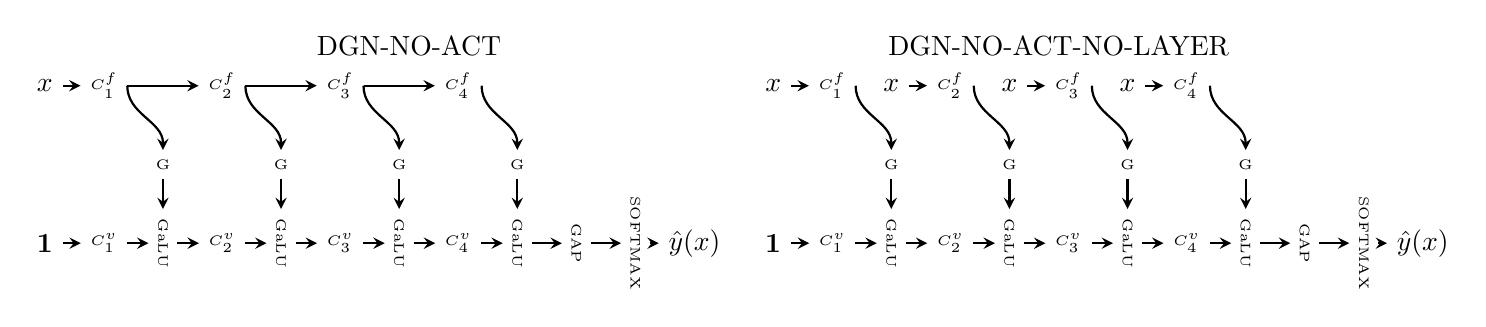
\begin{tikzpicture}
\node []  (fntext)at (-4.125,2) {DGN-NO-ACT};

%\node []  (output) at (7.5,1.5) {$\hat{y}(x)$};


\node [] (dgn1-f-c4) at (-3.5,1.5){\tiny{$C^{\text{f}}_4$}};
\node [] (dgn1-f-c3) at (-5,1.5){\tiny{$C^{\text{f}}_3$}};
\node [] (dgn1-f-c2) at (-6.5,1.5){\tiny{$C^{\text{f}}_2$}};
\node [] (dgn1-f-c1) at (-8,1.5){\tiny{$C^{\text{f}}_1$}};
\node [] (dgn1-input-f) at (-8.75,1.5){$x$};
\draw [-stealth,thick]   (dgn1-f-c3.east) -- (dgn1-f-c4.west);
\draw [-stealth,thick]   (dgn1-f-c2.east) -- (dgn1-f-c3.west);
\draw [-stealth,thick]   (dgn1-f-c1.east) -- (dgn1-f-c2.west);
\draw [-stealth,thick]   (dgn1-input-f.east) -- (dgn1-f-c1.west);



\node []  (dgn1-output) at (-0.5,-0.5) {$\hat{y}(x)$};

\node [rotate=-90] (dgn1-smax) at (-1.25,-0.5){\tiny{SOFTMAX}};
\draw [-stealth,thick]   (dgn1-smax.north)--(dgn1-output.west);

\node [rotate=-90] (dgn1-gap) at (-2,-0.5){\tiny{GAP}};
\draw [-stealth,thick]   (dgn1-gap.north)--(dgn1-smax.south);


\node [rotate=-90] (dgn1-galu-4) at (-2.75,-0.5){\tiny{GaLU}};
\draw [-stealth,thick]   (dgn1-galu-4.north)--(dgn1-gap.south);

\node [] (dgn1-v-c4) at (-3.5,-0.5){\tiny{$C^{\text{v}}_4$}};
\draw [-stealth,thick]   (dgn1-v-c4.east) -- (dgn1-galu-4.south);


\node [rotate=-90] (dgn1-galu-3) at (-4.25,-0.5){\tiny{GaLU}};
\draw [-stealth,thick]   (dgn1-galu-3.north) -- (dgn1-v-c4.west);

\node [] (dgn1-v-c3) at (-5,-0.5){\tiny{$C^{\text{v}}_3$}};
\draw [-stealth,thick]   (dgn1-v-c3.east) -- (dgn1-galu-3.south);


\node [rotate=-90] (dgn1-galu-2) at (-5.75,-0.5){\tiny{GaLU}};
\draw [-stealth,thick]   (dgn1-galu-2.north) -- (dgn1-v-c3.west);

\node [] (dgn1-v-c2) at (-6.5,-0.5){\tiny{$C^{\text{v}}_2$}};
\draw [-stealth,thick]   (dgn1-v-c2.east) -- (dgn1-galu-2.south);


\node [rotate=-90] (dgn1-galu-1) at (-7.25,-0.5){\tiny{GaLU}};
\draw [-stealth,thick]   (dgn1-galu-1.north) -- (dgn1-v-c2.west);


\node [] (dgn1-v-c1) at (-8,-0.5){\tiny{$C^{\text{v}}_1$}};
\draw [-stealth,thick]   (dgn1-v-c1.east) -- (dgn1-galu-1.south);


\node [] (dgn1-v-input) at (-8.75,-0.5){$\mathbf{1}$};




\node[] (dgn1-gating-4) at (-2.75,0.5){\tiny{G}};
\node[] (dgn1-gating-3) at (-4.25,0.5){\tiny{G}};
\node[] (dgn1-gating-2) at (-5.75,0.5){\tiny{G}};
\node[] (dgn1-gating-1) at (-7.25,0.5){\tiny{G}};

\draw [-stealth,thick]   (dgn1-f-c1.east) to[out=-90,in=90] (dgn1-gating-1.north);
\draw [-stealth,thick]   (dgn1-gating-1.south) -- (dgn1-galu-1.west);



\draw [-stealth,thick]   (dgn1-f-c2.east) to[out=-90,in=90] (dgn1-gating-2.north);
\draw [-stealth,thick]   (dgn1-gating-2.south) -- (dgn1-galu-2.west);




\draw [-stealth,thick]   (dgn1-f-c3.east) to[out=-90,in=90] (dgn1-gating-3.north);
\draw [-stealth,thick]   (dgn1-gating-3.south) -- (dgn1-galu-3.west);



\draw [-stealth,thick]   (dgn1-f-c4.east) to[out=-90,in=90] (dgn1-gating-4.north);
\draw [-stealth,thick]   (dgn1-gating-4.south) -- (dgn1-galu-4.west);

\draw [-stealth,thick]   (dgn1-v-input.east) -- (dgn1-v-c1.west);

%%%%%%%%%%%%%%%%%%%%%%%%%%%%%%%%%%%%%%%%%%%%%%%%%%%%%%%%%%%%%%%%%
\node []  (fntext)at (4.125,2) {DGN-NO-ACT-NO-LAYER};

%\node []  (output) at (7.5,1.5) {$\hat{y}(x)$};

\node [] (dgn-f-input) at (0.5,1.5){$x$};
\node [] (dgn-f-c4) at (5.75,1.5){\tiny{$C^{\text{f}}_4$}};

\node [] (dgn-f-x-4) at (5,1.5){$x$};


\node [] (dgn-f-c3) at (4.25,1.5){\tiny{$C^{\text{f}}_3$}};
\node [] (dgn-f-x-3) at (3.5,1.5){$x$};

\node [] (dgn-f-c2) at (2.75,1.5){\tiny{$C^{\text{f}}_2$}};
\node [] (dgn-f-x-2) at (2,1.5){$x$};

\node [] (dgn-f-c1) at (1.25,1.5){\tiny{$C^{\text{f}}_1$}};

\draw [-stealth,thick]   (dgn-f-input.east) -- (dgn-f-c1.west);
\draw [-stealth,thick]   (dgn-f-x-2.east) -- (dgn-f-c2.west);
\draw [-stealth,thick]   (dgn-f-x-3.east) -- (dgn-f-c3.west);
\draw [-stealth,thick]   (dgn-f-x-4.east) -- (dgn-f-c4.west);


\node []  (dgn-output) at (8.75,-0.5) {$\hat{y}(x)$};



\node [rotate=-90] (dgn-smax) at (8,-0.5){\tiny{SOFTMAX}};
\draw [-stealth,thick]   (dgn-smax.north) -- (dgn-output.west);
;
\node [rotate=-90] (dgn-gap) at (7.25,-0.5){\tiny{GAP}};
\draw [-stealth,thick]   (dgn-gap.north) -- (dgn-smax.south);



\node [rotate=-90] (dgn-galu-4) at (6.5,-0.5){\tiny{GaLU}};

\draw [-stealth,thick]   (dgn-galu-4.north) -- (dgn-gap.south);
\node [] (dgn-v-c4) at (5.75,-0.5){\tiny{$C^{\text{v}}_4$}};
\draw [-stealth,thick]   (dgn-v-c4.east) -- (dgn-galu-4.south);


\node [rotate=-90] (dgn-galu-3) at (5,-0.5){\tiny{GaLU}};
\draw [-stealth,thick]   (dgn-galu-3.north) -- (dgn-v-c4.west);


\node [] (dgn-v-c3) at (4.25,-0.5){\tiny{$C^{\text{v}}_3$}};
\draw [-stealth,thick]   (dgn-v-c3.east) -- (dgn-galu-3.south);


\node [rotate=-90] (dgn-galu-2) at (3.5,-0.5){\tiny{GaLU}};
\draw [-stealth,thick]   (dgn-galu-2.north) -- (dgn-v-c3.west);

\node [] (dgn-v-c2) at (2.75,-0.5){\tiny{$C^{\text{v}}_2$}};
\draw [-stealth,thick]   (dgn-v-c2.east) -- (dgn-galu-2.south);


\node [rotate=-90] (dgn-galu-1) at (2.0,-0.5){\tiny{GaLU}};
\draw [-stealth,thick]   (dgn-galu-1.north) -- (dgn-v-c2.west);

\node [] (dgn-v-c1) at (1.25,-0.5){\tiny{$C^{\text{v}}_1$}};
\draw [-stealth,thick]   (dgn-v-c1.east) -- (dgn-galu-1.south);


\node [] (dgn-v-input) at (0.5,-0.5){$\mathbf{1}$};


\node[] (dgn-gating-1) at (2.0,0.5){\tiny{G}};
\draw [-stealth,thick]   (dgn-f-c1.east) to[out=-90,in=90] (dgn-gating-1.north);
\draw [-stealth,thick]   (dgn-gating-1.south) -- (dgn-galu-1.west);


\node[] (dgn-gating-2) at (3.5,0.5){\tiny{G}};
\draw [-stealth,thick]   (dgn-f-c2.east) to[out=-90,in=90] (dgn-gating-2.north);
\draw [-stealth,thick]   (dgn-gating-2.south) -- (dgn-galu-2.west);



\node[] (dgn-gating-3) at (5,0.5){\tiny{G}};
\draw [-stealth,thick]   (dgn-f-c3.east) to[out=-90,in=90] (dgn-gating-3.north);
\draw [-stealth,thick]   (dgn-gating-3.south) -- (dgn-galu-3.west);


\node[] (dgn-gating-4) at (6.5,0.5){\tiny{G}};
\draw [-stealth,thick]   (dgn-f-c4.east) to[out=-90,in=90] (dgn-gating-4.north);
\draw [-stealth,thick]   (dgn-gating-4.south) -- (dgn-galu-4.west);

\draw [-stealth,thick]   (dgn-v-input.east) -- (dgn-v-c1.west);
	
\end{tikzpicture}


}
\end{minipage}
\end{minipage}
\caption{DGN}
\label{fig:dgn}
\end{figure}


The DGN performs only marginally poor compared to the DNN, and by successfully addressing the `black box'-ness issue in a DGN we will have both performance and interpretability. We now propose our novel \texttt{DGN-NO-ACT}  which disentangles the computations into (i) primal linear layer-by-layer computation, (ii) dual linear path-by-path computation and (iii) gating non-linearity which \emph{lifts} the computations from the primal to the dual. \texttt{DGN-NO-ACT} (right diagram in \Cref{fig:dgn}) is obtained by making a novel modification to the DGN (left diagram in \Cref{fig:dgn}) as follows:

1. We replace the ReLUs in the feature network with \emph{identity} maps, i.e., $I(q) = q$. Thus, in the \texttt{DGN-NO-ACT}, the transformation from input to the pre-activations is entirely linear. We call this \textbf{primal linearity}. The disentanglement happens because the ReLU  is completely removed.  

2. The value network of the DGN is linear in dual `path' variables. We call this \textbf{dual linearity} which stands for the fact that the value network computes path-by-path, and not layer-by-layer. As a result, presenting a $\mathbf{1}$ as input to the value network in \texttt{DGN-NO-ACT} does not degrade performance. The simplifications are : (i) $v_{\Tv}\in \R^{\text{total\,paths}}$ is a vector that does not depend on the input, and (ii) $\phi_{\Tf}(x)\in(0,1)^{\text{total\,paths}}$ is a  simple feature vector. In other words, the value network  learns the paths, and the feature network learns the activations of paths for each input.  While in each layer of the value network GaLUs and the linear operations are entangled, disentanglement happens in the path variables, and we do not have to worry about how learning happens layer-by-layer.

%3. The gates themselves serve the functionality of \emph{lifting} the computations from the primal to the dual, i.e., pre-activations trigger the gates which in turn activate the paths.

%\textbf{Significance.} The salient importance of the \texttt{DGN-NO-ACT} is that it clearly separates the layer-by-layer computations in the feature network and path-by-path computation in the value network. The importance of primal linearity is that we can now use standard linear algebra to `mathematically' interpret the linear transformations from the input to the pre-activations. Also, in the case of specific application domains such as `image classification', these transformations are `filter banks' which have been extensively studied with well known interpretations. The `mathematical' as well as domain specific interpretabilities obviate the need for `locally linear explanation using simpler models': the feature network is entirely linear and is itself simple. The importance of dual linearity is that it gives us a \emph{kernel} based `mathematical' interpretation in the \emph{infinite width regime}. 


%\textbf{DGN-NO-ACT(our model)}(see right diagram in \Cref{fig:dgn}). We replace the ReLUs in the feature network with \emph{identity} maps, i.e., $I(q) = q$. Thus, in the \texttt{DGN-NO-ACT}, the transformation from input to the pre-activations is entirely linear and is amenable to interpertation via standard spectral analysis using linear algebraic tools. The pre-activations trigger the gates, which then dictates the path activity. The value network is given only given $\mathbf{1}$ as input and hence $v_{\Tv}\in \R^{\text{total\,paths}}$ is a vector that does not depend on the input, and $\phi_{\Tf}(x)\in(0,1)^{\text{total\,paths}}$ is a very simple feature vector. % and the output $\hat{y}_{\text{DGN}}(x)=\ip{\phi_{\Tf}(x),v_{\Tv}}=\sum_{p}\phi_\Tf(x,p)v_\Tv(p)$ is equal to \emph{\textbf{the summation of `path value' weighted by the `path activations'}}. 
%Thus, the \texttt{DGN-NO-ACT} can be seen to disentangle the `primal linear' feature network which generates the gates, which in turn activate the paths in the value network which is the `dual linear'.

%\textbf{Remark.} Presenting the value network with $\mathbf{1}$ is very counter intutive, which will get justfied in theory as well as experiments in the next section. As a quick check, we the test accuracies of a DNN $4$ with convolutional layers and global-average-pooling (GAP), its corresponding DGN and \texttt{DGN-NO-ACT} on CIFAR-10 are {\bf{DNN: $80.4\%$,  DGN: $77.4\%$, \texttt{DGN-NO-ACT} : $74.5\%$}}.

%Since $\hat{y}_{\Theta}(x)=\ip{\phi_{x,\Theta},v_{\Theta}}$, during training, as $\Theta$ is learnt, both the NPFs and NPV are also learnt. To understand their roles better, $\phi_{x,\Theta}$ and $v_{\Theta}$ have to be separated.  This is achieved by the deep gated network (DGN) setup (see \Cref{fig:dgn}), which has two networks of \emph{identical architecture} namely the \emph{feature network} ($\Tf\in\R^{d^{\text{f}}_{\text{net}}}$) which holds the NPFs (i.e., the gating information) and the \emph{value network} ($\Tv\in\R^{d^{\text{v}}_{\text{net}}}$) which holds the NPV.  The combined parameterisation is denoted by $\Theta^{\text{DGN}}=(\Tf,\Tv)\in \R^{d^{\text{f}}_{\text{net}}+d^{\text{v}}_{\text{net}}}$.  The feature network is a DNN with ReLUs and the value network is a DNN with \emph{Gated Linear Units (GaLUs)} (terminology used in [\citenum{sss}]) whose output is the product of its pre-activation input $q^{\text{v}}(x)$and the external gating signal $G^{\text{f}}(x)$ (see \Cref{fig:dgn}). In \Cref{fig:dgn}, the main output of the DGN is $\hat{y}_{\text{DGN}}(x)$, while the other output $\hat{y}_{\text{f}}(x)$ is used to \emph{pre-train} the gates (see \Cref{sec:exp}).

